% Section content template for individual Educative lessons
% This file contains the actual content for a specific section
% Generated from Educative API section content

% Section: Requirements of a Distributed Messaging Queue’s Design
% Section ID: 5806944861814784
% Section Slug: requirements-of-a-distributed-messaging-queues-design
% Generated: 2025-12-07T20:57:40.133342

\subsection{Requirements}\label{WMDX0GYBv-mJ7IwlZZWYn}
\\
In a \textbf{distributed messaging queue}, data resides on several machines. Our aim is to design a distributed messaging queue that has the following functional and non-functional requirements.

\subsubsection{Functional requirements}\label{KP36CB7114DhAtEq_nS_K}
\\
Listed below are the actions that a client should be able to perform:

\begin{itemize}
\item
\protect\phantomsection\label{gmyh8KO8p1PZYIvB7ZrY0}
\textbf{Queue creation:} The client should be able to create a queue and set some parameters---for example, queue name, queue size(A queue size is the maximum number of messages a queue can contain. For example, Amazon's standard queue size is unlimited. However, for inflight messages, the size is limited to 120,000.), and maximum message size. MaxMessageSize
\item
\protect\phantomsection\label{nSTSnL3XyCvKXO3yl5Pi1}
\textbf{Send message:} Producer entities should be able to send messages to a queue that's intended for them.
\item
\protect\phantomsection\label{XctGuR3Rvpy602YsAFB69}
\textbf{Receive message:} Consumer entities should be able to receive messages from their respective queues.
\item
\protect\phantomsection\label{Lc4n3JjE0kF6V2tjE4bTA}
\textbf{Delete message:} The consumer processes should be able to delete a message from the queue after a successful processing of the message.
\item
\protect\phantomsection\label{phvQd8rWl3rd_mJu_HTsJ}
\textbf{Queue deletion:} Clients should be able to delete a specific queue.
\end{itemize}

\subsubsection{Non-functional requirements}\label{wHq2HcuSktQ-Twkr4ZYht}
\\
Our design of a distributed messaging queue should adhere to the following non-functional requirements:

\begin{itemize}
\item
\protect\phantomsection\label{MKospkOZGouADcZepOHvm}
\textbf{Durability}: The data received by the system should be durable and shouldn't be lost. Producers and consumers can fail independently, and a queue with data durability is critical to make the whole system work, because other entities are relying on the queue.
\item
\protect\phantomsection\label{R_i7PqRIrBQs11oOGnjlt}
\textbf{Scalability}: The system needs to be scalable and capable of handling the increased load, queues, producers, consumers, and the number of messages. Similarly, when the load reduces, the system should be able to shrink the resources accordingly.
\item
\protect\phantomsection\label{5UCr1MIzTW20lVscK37w1}
\textbf{Availability}: The system should be highly available for receiving and sending messages. It should continue operating uninterrupted, even after the failure of one or more of its components.
\item
\protect\phantomsection\label{P3Wd7oHBweivgneKwmFkj}
\textbf{Performance:} The system should provide high throughput and low latency.
\end{itemize}

\subsection{Single-server messaging queue}\label{V680K8ql0ZeaMPxrkpRHJ}
\\
Before we embark on our journey to map out the design of a distributed messaging queue, we should recall how queues(Such a queue is also called a bounded queue, due to its fixed size within the system.) are used within a single server where the producer and consumer processes are also on the same node. A producer or consumer can access a single-server queue by acquiring the locking mechanism to avoid data inconsistency. The queue is considered a critical section where only one entity, either the producer or consumer, can access the data at a time.
\\
However, several aspects restrain us from using the single-server messaging queue in today's distributed systems paradigm. For example, it becomes unavailable to cooperating processes, producers and consumers, in the event of hardware or network failures. Moreover , performance takes a major hit as contention on the lock increases. Furthermore, it is neither scalable nor durable.

\begin{figure}[htbp]
 \centering
 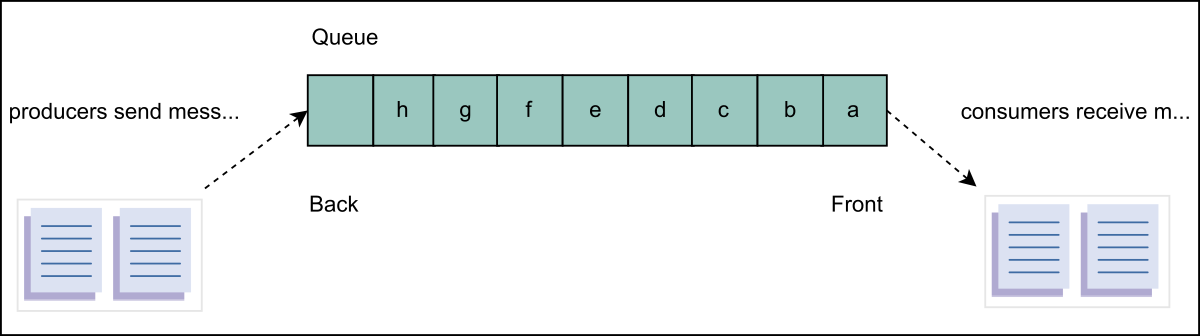
\includegraphics[width=0.5\textwidth]{Images/chapter_17/section_5806944861814784/5303608228970496.png}
 \caption{Multiple producers and consumers interact via a single messaging queue}
\end{figure}

\begin{quote}
\textbf{Quiz:}
\textbf{Question 1:} Can we extend the design of a single-server messaging queue to a distributed messaging queue?
\textbf{Answer:} A single-server messaging queue has the following drawbacks: 1. High latency: As in the case of a single-server messaging queue, a producer or consumer acquires a lock to access the queue. Therefore, this mechanism becomes a bottleneck when many processes try to access the queue. This increases the latency of the service. 2. Low availability: Due to the lack of replication of the messaging queue,

the producer and consumer process might be unable to access the queue in events of failure. This reduces the system's availability and reliability. 3. Lack of durability: Due to the absence of replication, the data in the queue might be lost in the event of a system failure. 4. Scalability: A single-server messaging queue can handle a limited number of messages, producers, and consumers.

Therefore, it is not scalable. To extend the design of a single-server messaging queue to a distributed messaging queue, we need to make extensive efforts to eliminate the drawbacks outlined above.
\end{quote}

\subsection{Building blocks we will use}\label{fLoEbvk6nnXHsapun-GUm}

The design of a distributed messaging queue utilizes the following building blocks:

\begin{figure}[htbp]
 \centering
 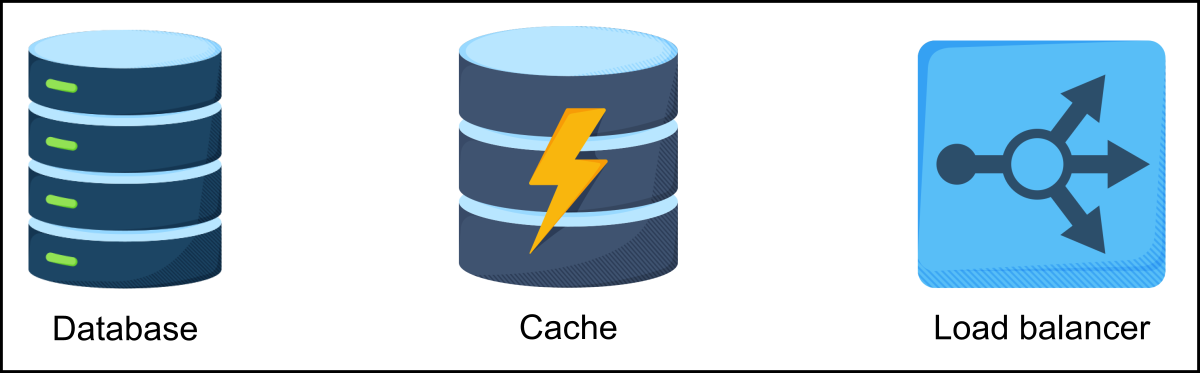
\includegraphics[width=0.5\textwidth]{Images/chapter_17/section_5806944861814784/5761017267486720.png}
 
\end{figure}

\begin{itemize}
\item
\protect\phantomsection\label{DcSZyWLAM5Eh93xca2ZU9}
\href{https://www.educative.io/courses/grokking-the-system-design-interview/introduction-to-databases}{\textbf{Database(s)}} will be required to store the metadata of queues and users.
\item
\protect\phantomsection\label{gXPqu1uY4ukH7pxj3O46I}
\href{https://www.educative.io/courses/grokking-the-system-design-interview/system-design-the-distributed-cache}{\textbf{Caches}} are important to keep frequently accessed data, whether it be data pertaining to users or queue metadata.
\item
\protect\phantomsection\label{-Q5fq2blcR7q74LvBgohv}
\href{https://www.educative.io/courses/grokking-the-system-design-interview/introduction-to-load-balancers}{\textbf{Load balancers}} are used to direct incoming requests to servers where the metadata is stored.
\end{itemize}
\\
In our discussion on messaging queues, we focused on their functional and non-functional requirements. Before moving on to the process of designing a distributed messaging queue, it's essential for us to discuss some key considerations and challenges that may affect the design.\\
\strut \\

% End of section content